\documentclass[man]{apa}
\usepackage{listings}
\usepackage{courier}

\title{JavaScript}
\author{Jeffrey W. Allen}
\affiliation{University of North Alabama\\ Florence, Alabama}
\abstract{

This paper explores the JavaScript high-level, untyped, dynamic, interpreted programming language. First, a brief history of this this language is presented. This is then followed by in depth discussions of how the JavaScript programming language interfaces with computers. Throughout this paper, JavaScript may sometimes be referred to as JS.

}

\acknowledgements{Patricia Roden}

\begin{document}
\maketitle

%============================================================================================================================
%==============================================    1     ====================================================================
%============================================================================================================================
\section{History}
%============================================================================================================================
%============================================================================================================================
%============================================================================================================================

%http://www.power-ecmascripting.com/javascript.htm

% Who what when where why
% 
Back in the early 1990's, there was an eruption of people that began using the web. It was almost as if the printing press was yet again recreated. Information was being shared amongst large numbers of people like never before. This was because of the introduction of new interfaces created specifically for these users to browse the web. The two main interfaces created were the graphical web browser, along with the Common Gateway Interface (CGI). The graphical web browser migrated web browsing done from the command line environment to a more intuitive environment which provided buttons and tools such as automatic URL lookups. With introduction of the Common Gateway Interface however, this allowed HTML (hypertext markup language) to request programs to be executed on the server.


This idea of clients continuously requesting information from the servers in order for something small to change on the client's computer became old though. A few companies such as Sun Cooperation, Microsoft, and NetScape, quickly came to the realize graphical web browsers lacked the ability to make computation associated with the rendered HTML. Sun's coopreration which owned the stable language Java, attempted to implement Java Applets that ended up being an overall failed design. NetScape, a company known for its own graphical web browser the NetScape Navigator, succeeded with decision of hiring a programmer named Brendan Eich to currate its solution for client side HTML computation, named Mocha, released in September of 1995. It was quickly thereafter renamed to LiveScript in September of 1995, and then renamed again to what we know now as JavaScript in December of that year. Microsoft saw the success JavaScript was having. So they used that design as a base for their own scripting language, named JSscript.

% ECMAScript
With the fallout of Java Applets, and the rise of Microsoft's own flavor of a scripting language, Netscape quickly seeked to attain uniformity for its language by wanting solid language specification. Being that a language is an abstract idea, it is confusing for programmers to work together when no rules are specified. So This is where these cooprerations offered the language up for standardization in 1996 to the European Computer Manufactuers Association (ECMA). Bickering ensued on what official name the standard should be released on, so in June of 1997, the language standard's name was given a default of "Standard ECMA-262 (ECMAScript core)". This lead to the Internation Standards Organization (ISO) to also recognize ECMAScript as an international standard ISO/IEC 16262. It is updated regularly, with this paper putting emphasis on the ECMAScript 5.1.


%============================================================================================================================
%==============================================    2     ====================================================================
%============================================================================================================================
\section{Design Goals}
%============================================================================================================================
%============================================================================================================================
%============================================================================================================================

According to the ECMAScript 5.1 manual, ECMAScript (which emphasized as being simply a standardization reference to JS) was originally designed to be a web scripting language. A mechanism to which animates web pages in browsers to perform computation as a part of a Web-based client-server architecture. This follows closely to what Brendan Eich in 2008, a lead developer of JavaScript who now works for Mozilla, explained. This is when he was asked the question "What was your main goal in developing JavaScript?" To where he replied, "The idea was to make something that Web designers, people who may or may not have much programming training, could use to add a little bit of animation or a little bit of smarts to their Web forms and their Web pages." With this overall goal in mind, it inherently created issues related to design trade-offs. As will be seen throughout this paper, many decisions in the design were in favor of allowing a programmer to execute programs quickly. This comes at the expense of a program reliable.

% Language Recognizer
In the battle between reliability and execution efficiency, it is apparent the latter won. One of the main reasons being Eich chose the language implementation of interpretation. This is where the source code is interpreted by a program which and executed directly on the machine. No translation occurs and object code is not produced for the program at all. The choice of the language being purely interpreted was driven by of one of the reasons Java Applets failed. Which was the heavy nature its intermediate code generator.

Java Applets took a hybrid approach of complitation and interpretation by translating its high-level language programs to intermediate language machine code to run its programs. Any compilation on the native machine at all made it slow and difficult for users to just browse web pages. Users simply did not want to wait for a program to be translated to native machine code, but rather quickly begin its execution. This decision also allowed JS to have even greater platform independance. The interpreter is usually embedded into popular graphical web browsers such as Google's V8 interpreter inside Google Chrome's browser, and Mozilla's Spidermonkey inside of Firefox.

The draw-backs of this though is that it is 10 to 100 times slower than a program which is compiled. Slowness is due to complexity of decoding high-level statements. To which each time the interpreted JS program is ran, it must be decoded every single time. Another disadvantage includes the fact the source program requires more space. Although Google's V8 engine attempts to resolve this by making multiple passes through a source program to reduce redundancy of defining statements.

%============================================================================================================================
%==============================================    3     ====================================================================
%============================================================================================================================
\section{Syntax}
%============================================================================================================================
%============================================================================================================================
%============================================================================================================================
\lstset{ % basics
	basicstyle=\small,
	tabsize=4
}


% Intro to syntax
% Where the syntax comes from
Syntax describes the actual form of the language's expressions, statements, and program units. The standardized structure of statements can be found in the language's specification, ECMAScript. In a 2008 interview, Brendan Eich explains that "we were pushing it (JavaScript) as a little brother to Java, as a complementary language like Visual Basic was to C++ in Microsoft’s language families at the time. And it took off. We got it out in time." This is one of the main reasons JavaScript's own case-sensitive syntax heavily resembles that of Java and C.

% Semantics, % Describing Syntax: EBNF which has been translated into Syntax Diagrams
A language's syntax can be combined in different ways in order to form different semantics. A language's semantics describe  actual meaning of these syntactic constructs. ECMAScript 5.1 utilizes the EBNF (Extended Backus-Naur Form) metalanguage in order to describe its own syntax and semantics. Productions are represented as text residing on the left-hand side (LHS) of the the assignment statement, represented with two colons, followed by a list of references to mixture of tokens, lexemes, and references to other abstractions. Douglas Crockford, a noteable individual that is quite active the JavaScript community created syntax diagrams which graphically represents these productions. This is included in Appendix $A$.

% Language recognizer and generator
As stated before, this language is interpreted. Google has developed its own interpreter, the V8 Engine, which is an open-source project written in C. V8 analyzes syntax by creating its very own abstract syntax tree from the source code with a file aptly named "AST.h", which stands for Abstract Syntax Tree. This checks to see if the code written is in fact valid JavaScript. The example below contains the necessary code to check if a JS \texttt{for} statement is valid.

%----------------------For statement language analysis-------------------------
\lstinputlisting[language=C++, label={Abstract Syntax Tree}, firstline=830, lastline=886]{v8_ast.c}

%============================================================================================================================
%==============================================    4     ====================================================================
%============================================================================================================================
\section{Expressions and Assignment Statements}
%============================================================================================================================
%============================================================================================================================
%============================================================================================================================

% Intro
According to Sebesta (2012), "Expressions are the fundamental means of specifying computations in a programming language." Simply put, an expression in JS is a phrase which the interpreter can evalute. It is further explained that "The precondition and postcondition of an assignment statement together define precisely its meaning" (p. 150). These two concepts provide the building blocks for how results are produced by programs and algorithms. In this section, it will be explained how these fundamental concepts of computing are accomplished by JavaScript.

%****need transition*****
A paradigm in programming describes the style of structure and elements of computer programs. JavaScript itself utilizes multiple paradigms. It can be either object-oriented, imperative, and even functional. Object-oriented, which is usually paired with the imperative paradigms, allow for the state of a program to change based on the sequential assignment of objects. These objects can consist of abstract data types which can inherit from other objects to which attributes can be dynamically bound. The lesser used functional paradigm allows JS programs to produce results without the use of assignment statements of variables. Programs instead are controlled soley by function applications and conditional expressions. An example of this can be seen the way JavaScript's functions are treated first class objects.

% example program


% Expressions
 This will produce a value. The syntax diagram below describes an expression.

% Insert expression syntax diagram.

% Assignment Statements
When an assignment occurs in JavaScript, both a variables type and value is bound. This is just the nature of dynamic typing. JavaScript does follow the current trend of using a single equal sign for assignment. It also supports compound assignment operators, conditional targets, unary assignment as well. For example:

%----------------------Compound operator example-------------------------
\lstinputlisting[language=C++, label={Compound Operator Example}, firstline=91, lastline=95]{program.js}

% Operator precedence: 16 --- Associativity operators
All the operators from Java are included in JS. There also includes two new equality operators, \texttt{===} and \texttt{!==} operators. These check to see if the two operands on either side of have the same type and same value. According to Crockford, these new operators do not coerce values of the operands being checked if they are of different types, the way the old \texttt{==} and \texttt{!=} operators do.

%----------------------Equivalence operator-------------------------
\lstinputlisting[language=C++, firstline=79, lastline=87]{program.js}

To understand the evaluation of an expression in JavaScript, it must first be understood the precedence in which operators are assigned. The operarators which have the highest precedence over all others are the refinement and invocation operators. These are things like the \texttt{.}, \texttt{[]}, and \texttt{()} operators. The next set of operators evaluated by JavaScript interpreter are unary operators. These include operators such as \texttt{delete}, \texttt{new}, \texttt{typeof}, \texttt{+}, \texttt{-} and \texttt{!}. Multiplication, division, and remainder operatations are all viewed by the interpeter as having the same precedence. The next level of precedence below these operators include addition, concatentation and subtraction operations. These are followed by the inequality operators, such as \texttt{>=}, \texttt{<=}, \texttt{>}, and \texttt{<}. Equality operators, such as the ones in the example above, are evaluated next. The logical operations are evaluated next. Where the logical and operation has precedence over the logical or. Where lastly, the ternary operator is evaluated. It is important to note that JS does not support overloading operators.

%============================================================================================================================
%==============================================    5     ====================================================================
%============================================================================================================================
\section{Data Types}
%============================================================================================================================
%============================================================================================================================
%============================================================================================================================

JavaScript has a set of primitive data types and one complex data type. The primitive data types are not defined in terms of other types. These include \texttt{number}, \texttt{string}, \texttt{boolean}, \texttt{undefined}, and \texttt{null}. The complex data type \texttt{object} is a collection of properties, where each property is a name-value pair. 

The only numeric type in this language is \texttt{number}. All numbers in JavaScript are represented in memory as IEEE-754 floating-point format. All integers between $ -2^{53} $ to $ 2^{53} $ can be represented in memory exactly. Floating-point literals, or real numbers, however causes problems when relation and arithmetic operation occurs. This is because values like $ 0.1 $ cannot be represented in memory precisely. The following example shows how this can cause problems.

%----------------------Real numbers-------------------------
\lstinputlisting[language=C++, firstline=98, lastline=102]{program.js}

The \texttt{string} type allows for JS to represent text. It uses a 16-bit unsigned value used to represent a single unit of text. The UTF-16 ecoding of the Unicode character set is used to decipher which character is which. For example, the character "a" in JavaScript is actually the hexidecimal number 0x0061. Variables can be assigned literal values of strings by enclosing characters inside of quotes. These can be single, or double quoted. Explained later in this chapter, relational operations are made easier, such as pattern matching, with the the regular expression object.

Next, the \texttt{boolean} data type. It is the simplest data type in JS. This is because they can only be either one of two values, true or false. This is usually represented in memory as a single byte with either a value of 0 or value of 1.

The last two primitivie data types \texttt{undefined} and \texttt{null} are special. These two keywords in the language evalute to indicate there is no value. However, a curious event occurs when the \texttt{typeof} operator, an operator which returns the parameter's type as a string value, is used on \texttt{null}. The type object is returned. So in reality, it is a special type of object, but in real-world applications it is simply a method for explaining there is no value.

The last data type explained in this section is \texttt{object}. Rather than a single value being associated with this type, an object is a compound value. It is an unordered collection of properties with eaching having a name, and value associated with that name. A more common name for this data structure an associative array, or dictionary.

This is where JavaScript greatly showcases its object-oriented abilities. Abstraction, encapsulation, inheritence and polymorphism are all attained through use of this data type. It must be carefully observed the way inheritence is executed in this language though. The object which is inherited from is named a "prototype". Unlike in Java and C++ though, once an object inherits from its prototype, it is viewed as its own entity. This means when an object inherits all properties from its prototype, and the properties of the prototype is modiefied in any way (deleted, added, ect.), it does not affect the child object.

Arrays are a special type of object. An array is untyped, meaning that each element may be of a different type. The elements in this object are ordered, beginning at the 0 index. Theses arrays described as being heap-dynamic. This means the binding of subscript ranges and storage allocation is dynamic. They have the ability to change any number of times during the lifetime of the array. When attemptting to access and index which does not exist in an array, \texttt{undefined} is returned. This is common in sparse arrays, where there exist gaps between the indices of elements.

A wide variety of operations can be executed on an array. JavaScript 1.8 supports: addition of elements, addition of other arrays, deletion of elements, slicing or splicing, reversing, sorting and modification of elements can be done. There is also an operation which returns the length of the array, suitably named \texttt{length}. It is later explained how arrays can be used to achieve stacks and queues. %pg 223 in the complete javascript reference.

%============================================================================================================================
%==============================================    6     ====================================================================
%============================================================================================================================
\section{Data Structures}
%============================================================================================================================
%============================================================================================================================
%============================================================================================================================

JSON.

ECMAScript 6 will introduce classes.

%============================================================================================================================
%==============================================    7     ====================================================================
%============================================================================================================================
\section{Conditionals}
%============================================================================================================================
%============================================================================================================================
%============================================================================================================================

Conditional statements allow for the flow of a program to differ. As previously stated by Brendan Eich, JavaScript closely resembles Java. So with Java being an imperative language, computation is accomplished by assigning results of evaluted expressions to variables. Sometimes though, evaluations of statements need be alternatively chosen based on certain conditions. This concept gives programs power and flexibility by allowing different paths to be chosen and allowing for repitition of statements. In order for a program to decide the pathway and number of repitition iterations, logical control statements, counter controlled statements, or a combonation of the two are used.

Path selection of a program is based on selection statements. These provide the means of allowing to choose between two or more execution paths of a program. There exist two-way selection statements, along with multiple-selection statements. The two-way selection statements in JavaScript include \texttt{if}, \texttt{if-else}, \texttt{if-elif}, and \texttt{switch}. All of these statements change the flow of the program based on whether an expression evalutes \texttt{true} or \texttt{false}.

Flow control statements which provides repetition functionality to a program are called iterative statements. These can be contrived of a single statement, or or a collection of statements to be executed 0, one, or more times. Today, they are mostly referred to as loops. These include the \texttt{while} loop, and \texttt{do-while}, \texttt{for} loop. The only difference between the \texttt{while} and \texttt{do-while} loops is the fact \texttt{while} is entry controlled opposed to exit controlled like \texttt{do-while}.

According to Douglas Crockford, \texttt{false} values of expressions are defined. To which all other values are true. False values include the literals \texttt{false}, \texttt{null}, and \texttt{undefined}. Along with those values, the empty string \texttt{''}, the number \texttt{0}, and the number \texttt{NaN} also declare an expression to be false. With all other values being true. Even the string '\texttt{false}'.

%============================================================================================================================
%==============================================    8     ====================================================================
%============================================================================================================================
\section{Subprograms}
%============================================================================================================================
%============================================================================================================================
%============================================================================================================================

%	Intro

Subprograms in JavaScript are only known as functions. Even though some subprograms should be called procedures, in that some are simply a collection of statements that define parameterized computations, subprograms are named functions in JS. These special objects are able to be defined only once in the program, and have the ability to be invoked any number of times. JavaScript's function headers begins with the reserved word \texttt{function}, followed by an optional name, and an invocation expression. The invocation expression is made up of two parenthesis \texttt{()} that contain optional parameters, and a curly braces \texttt{{}} that wrap around statements, which make up the function's body.

A definition may include a list of identifiers, called parameters, that are used as local variables throughout the function's lifetime. When too many arguments are passed into a function's parameter list, they are ignored. Conversely, when there are not enough arguments passed into a function, they remaining parameters are assigned the value \texttt{undefined} in the function.

An interesting note about functions in JavaScript is that they are automatically brought to the top of the scope in which they are defined in. \textit{Hoisting} is the official term of this action upon functions. Hoisting allows functions to be called upon before they are defined in the scope they exist in. An example can be seen here:

%----------------------Hoisted function-------------------------
\lstinputlisting[language=C++, firstline=114, lastline=119]{program.js}

% Fundamentals
% Design issues
% Local referencing

Functions in this language can be either a statement or an expression. This is because they are treated as objects, known commonly as first class functions. This fact entails the ability for a whole function assigned the the value of another object. When an object contains a function, it is known as that object's method. When a function is invoked on, or even through an object, that object is a assigned the special property of being the function's invokation context. Therefore, the object is known in the function's environment as the value \texttt{this}.

The definition of a variable in a function is referred to as its referencing environment. Local variables, such as \texttt{this}, can either be defined statically or dynamically. JavaScript uses stack dynamic local variables. The main advantage of this decision is that storage is bound a variable when the program begins and unbound when the function finishes. This allows functions to be nested within each other, opening up the opportunity for recursion. 

JavaScript's decision of defining variables as stack-dynamic, like with many other decisions that must be made when designing a programming language, created trade-offs. The overhead of memory allocation, initialization and deallocation when stack-dynamic variables is one trade-off. Another trade-off based on this decision is that variables must always be referenced indirectly. In the next section "Parameter Passing", it is seen how JavaScript's variables directly affected by this decision when it also observes parameters that are passed-by-sharing.

% closures. Check Dougs book.
An explanation of closures should help clear up any confusion in understanding referencing environments. A closure is the term for a subprogram and the referencing environment where it was initially defined. Excellent news related to this concept is that emulation of private data members and methods of an object can be achieved. The trade-off is that performance is hindered where is an increase in both memory consumption and processing time. An example of this concept is demonstrated in the following code.

%----------------------Closures-------------------------
\lstinputlisting[language=C++, firstline=122, lastline=140]{program.js}

The focus in this program is the \texttt{object} candy. There also must be emphasis drawn to the \texttt{()}, or invocation expression, on the last line. The invocation expression allows the function to return an object that contains two methods. Anonymous function 1 is the closure of the variable flavor, along with anonymous functions 2 and 3, \texttt{changeFlavor} and \texttt{getFlavor}. To conclude this example, it is seen with the print statements that the main program does not have access to the variable flavor. This is because it is out of the scope of the main program. Only the methods for that object have the privilege of accessing that variable.

% design issues for functions
JavaScript is very lazy in protecting its users from creating side effects with functions. Side effects are indeed a normal occurrence with the dependence on global variables, such as HTML's \texttt{window} element for instance. With this language being untyped, there is no specification of the value's type returned from a function. Yet, JS functions have the restriction of only being able to return one value. The easy workaround for returning more than one value though is to return an array, which is untyped.

% user-defined overloaded operators
Subprograms in JavaScript do not support the ability to be overloaded. If two functions are declared with the same name in both headers of the functions, invokation of the function that was defined last will be executed. Along with subprograms having the restriction that they are unable to be overloaded, operators also adhere to this limitation. This constraint increases readability in the language by a minimizing the amount of referencing a programmer must do in order to understand its newly adopted semantics.

% callback functions
% coroutines

%============================================================================================================================
%==============================================    9     ====================================================================
%============================================================================================================================
\section{Parameter Passing}
%============================================================================================================================
%============================================================================================================================
%============================================================================================================================

As explained before, a parameter of subprogram (referenced interchangeably as a function in this section) is an interface a calling program uses to allow subprograms to access their data. There are many details to consider in any programming language associated with the way data is transferred from an outside environment in order to execute. In this section, the details are uncovered about how JS in particular attains access to the data it needs using parameters.


The parameters of a function in JS are positional parameters. A calling program who provides an array of arguments to a subprogram, delimited by commas, are known in the subprogram's environment by the position they were received. For example, a main program calls the function with the argument values of all type \texttt{Number}, with values 1, 2, and 3 like so \texttt{funct(1,2,3)}. In the subprogram's environment, the first parameter's value will be 1. The second would be 2. While the third parameter having the value 3. 

As explained in the previous section, when the number of arguments exceeds the amount defined in function's formal parameter list, they are ignored. Passing in less defaults all remaining parameters to undefined. 

There are multiple ways to to accomplish the goal of transmitting data to subprogram. The semantics JavaScript has chosen is a  Parameters are pass-by-value-result. This is a hybrid method of pass-by-value, and pass-by-result. 



,, and even passing other subprograms as a parameter to another subprogram.

Local variables are declared

Of all the parameter-passing methods there are, JavaScript utilizes the "pass-by-sharing".
% parameter passing
%Slide 8. Positional. Formal parameters are used. Positional parameters. Call-by-sharing.

It is obvious in this langauge that parameters are not checked for their types.


%============================================================================================================================
%==============================================    10     ===================================================================
%============================================================================================================================
\section{Data Abstractions}
%============================================================================================================================
%============================================================================================================================
%============================================================================================================================

Abstraction is a view or representation of any entity that includes only the most signifcant attributes.

An instance of an abstract data type is called an object.

%============================================================================================================================
%==============================================    11     ===================================================================
%============================================================================================================================
\section{Concurrency}
%============================================================================================================================
%============================================================================================================================
%============================================================================================================================

Ajax programming.

%============================================================================================================================
%==============================================    12     ===================================================================
%============================================================================================================================
\section{Recursion}
%============================================================================================================================
%============================================================================================================================
%============================================================================================================================

Yes.

%============================================================================================================================
%==============================================    13     ===================================================================
%============================================================================================================================
\section{Exception Handling}
%============================================================================================================================
%============================================================================================================================
%============================================================================================================================

JavaScript does exception handlers. These are special processing events that attempt to control the interference of normal program flow. The exception object

%----------------------Exception Example-------------------------
\lstinputlisting[language=C++, firstline=67, lastline=76]{program.js}

Interesting enough though, JavaScript does not raise errors when overflow or underflow occurs. Only the values \texttt{infinity}, \texttt{-infinity}, or simply \texttt{NaN} (Not a Number) are printed out when events like division by $ 0 $ occurs.

%============================================================================================================================
%==============================================    14     ===================================================================
%============================================================================================================================
\section{Input/Output}
%============================================================================================================================
%============================================================================================================================
%============================================================================================================================

% Explain how APL needed a specia keyboard

% Script tags

% including .js files

% Buttons

% Text boxes

% Select buttons

% Radio buttons


%============================================================================================================================
%==============================================    15     ===================================================================
%============================================================================================================================
\section{Unusual Features}
%============================================================================================================================
%============================================================================================================================
%============================================================================================================================

%============================================================================================================================
%==============================================    16     ===================================================================
%============================================================================================================================
\section{Contributions to the Programming Language Landscape}
%============================================================================================================================
%============================================================================================================================
%============================================================================================================================

%============================================================================================================================
%============================================================================================================================
%============================================================================================================================
\section{References}
%============================================================================================================================
%============================================================================================================================
%============================================================================================================================



%============================================================================================================================
%============================================================================================================================
%============================================================================================================================
\section{Personal Reflection}
%============================================================================================================================
%============================================================================================================================
%============================================================================================================================

	Consider the environment this programming language is being exposed to. Idiocy building on idiocy isn’t something you want, and is very hard to decipher between intelligence when surrounded by bad. I hesitate to fall head over heels in love with this language.

	People in the previous years had to wait a whole day for their code to compile. Waiting a whole day to find out there is a semi-colon missing provided incentive to pay attention to detail. JavaScript however is an interpreted language. This language’s interpreter is being supported by a majority of browsers being used by people today.

\end{document}


%,,,,,,,,,,,,,,,,,,,,,,Need to put in,,,,,,,,,,,,,,,,,,,,,,,,
% Table 4-1. JavaScript operators.


% \begin{figure}[h]
	
% 	\centering
% 		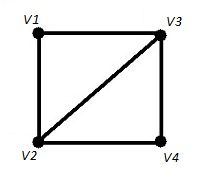
\includegraphics[width=0.25\textwidth]{figure1}
% 	\caption{Figure 1}

% \end{figure}

%============================================================================================================================
%============================================================================================================================
%============================================================================================================================% 
%\section{Adjacency matrix for $A$} 
%============================================================================================================================
%============================================================================================================================
%============================================================================================================================

% \[ A = \left( \begin{array}{cccc}
% 0 & 1 & 1 & 0 \\
% 1 & 0 & 1 & 1 \\
% 1 & 1 & 0 & 1 \\
% 0 & 1 & 1 & 0 \end{array} \right)\] 

%============================================================================================================================
%============================================================================================================================
%============================================================================================================================% 
%\section{$A^2$ and $A^3$}
%============================================================================================================================
%============================================================================================================================
%============================================================================================================================

% \[ A^2 = \left( \begin{array}{cccc}
% 2 & 1 & 1 & 2 \\
% 1 & 3 & 2 & 1 \\
% 1 & 2 & 3 & 1 \\
% 2 & 1 & 1 & 2 \end{array} \right)\] 

% \[ A^3 = \left( \begin{array}{cccc}
% 2 & 5 & 5 & 2 \\
% 5 & 4 & 5 & 5 \\
% 5 & 5 & 4 & 5 \\
% 2 & 5 & 5 & 2 \end{array} \right)\] 

% \pagebreak

% \subsection{What values in $A^n$ tell about the graph in Figure 1 & proving your claim for $A^2$} 

% The $n$ in the expression $A^n$ represents the amount of edges that must be used in order to travel between one  node, to another.
% The adjacency matrix for $A^1$ represents $0$ paths between $V_1$ and itself. In the adjacency matrix $A^2$, there are
% $2$ possible paths from $V_1$ to itself utilizing 2 edges.

%============================================================================================================================
%============================================================================================================================
%============================================================================================================================% 
%\section{Compute the eigenvalues and eigenvectors for $A$}
%============================================================================================================================
%============================================================================================================================
%============================================================================================================================

%   \begin{center}
%   \textbf{Eigenvalues}
%   \end{center}

%   \begin{center}
%   \begin{tabular}{ c c c p{5cm} }
%     $\lambda_1$ & $\rightarrow$ & $\frac{1}{2}(1+\sqrt{17})$ \\        
%     $\lambda_2$ & $\rightarrow$ & $\frac{1}{2}(1-\sqrt{17})$ \\
%     $\lambda_3$ & $\rightarrow$ & -1 \\
%     $\lambda_4$ & $\rightarrow$ & 0 \\
%   \end{tabular}
%   \end{center}

%   \begin{center}
%   \textbf{Eigenvectors}
%   \end{center}

%   \begin{center}
%   $\vec{x}_1 = \begin{pmatrix}1\\\frac{1}{4}(1 + \sqrt{17})\\\frac{1}{4}(1 + \sqrt{17})\\1\end{pmatrix}$
%   $\vec{x}_2 = \begin{pmatrix}1\\\frac{1}{4}(1 - \sqrt{17})\\\frac{1}{4}(1 - \sqrt{17})\\1\end{pmatrix}$
%   $\vec{x}_3 = \begin{pmatrix}0\\-1\\1\\0\end{pmatrix}$
%   $\vec{x}_4 = \begin{pmatrix}-1\\0\\0\\1\end{pmatrix}$
%   \end{center}

% \subsection{Importance of eigenvalues and eigenvectors to graph}

% We observed that there is one zero, one positive, and two negative eigenvalues for the adjacency matrix $A$.
% The importance of these values related to the graph can be used to determine the structure of the graph.
% For this graph, 

% \pagebreak

% \begin{figure}[h]
% 	\centering
% 		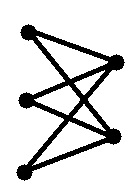
\includegraphics[width=0.25\textwidth]{figure2}
% 	\caption{Figure 2}
% \end{figure}

%============================================================================================================================
%============================================================================================================================
%============================================================================================================================% 
%\section{Draw the adjacency matrix $A$ for Figure 2}
%============================================================================================================================
%============================================================================================================================
%============================================================================================================================

% \[ \left( \begin{array}{ccccc}
% 0 & 1 & 0 & 1 & 0 \\
% 1 & 0 & 1 & 0 & 1 \\
% 0 & 1 & 0 & 1 & 0 \\
% 1 & 0 & 1 & 0 & 1 \\
% 0 & 1 & 0 & 1 & 0 \end{array} \right)\] 

%============================================================================================================================
%============================================================================================================================
%============================================================================================================================% 
%\section{Figure 2 Cycles} 
%============================================================================================================================
%============================================================================================================================
%============================================================================================================================
% \subsection{Amount of 2-cycles for the left-hand and right-hand vertices}

% \centerline{Left-hand: 6}
% \centerline{Right-Hand: 6}

% \subsection{Amount of 4-cycles for the left-hand and right-hand vertices} 

% \centerline{Left-hand: 6}
% \centerline{Right-Hand: 4}

% \subsection{Amount of 6-cycles for the left-hand and right-hand vertices} 

% \centerline{Left-hand: 0}
% \centerline{Right-Hand: 0}


